% !TEX root = ../thesis.tex

\chapter{Preliminaries}
\label{sec:preliminaries}

This chapter introduces the general notions and terminologies that will be used throughout this thesis, which are based on \cite{holldobler2009logic, lloyd2012foundations}. We start with Section~\ref{sec:preliminaries:abduction} by introducing some of the basic concepts about logic programming, the three-valued semantics and the weak completion semantics which are necessary to understand the abductive framework. Then in Section~\ref{sec:preliminaries:cn} we introduce some of the basic concepts about connectionist networks and recurrent connectionist networks which are going to be used later for the generation of candidate explanations for the abductive framework. In particular, we will introduce the architecture and main concepts of Jordan and Elman networks.

\section{Abduction under the Weak Completion Semantics}
\label{sec:preliminaries:abduction}

We assume the reader to be familiar with logic and logic programming. In the sequel, we will only consider propositional programs. If a program $\CalP$ is not propositional, then a propositional program $\CalP'$ corresponding to $\CalP$ can be obtained by grounding the program $\CalP$. We assume that each non-propositional program contains at least one constant symbol. The language $\CalL$ underlying a non-propositional program $\CalP$ contains precisely the predicate and constant symbols occurring in $\CalP$, and no others. Therefore, the following definitions can also be applied to programs which are not propositional. In those cases, we only need to compute the respective grounded program beforehand and reason with respect to it.

Therefore, we consider an \textit{alphabet} that consists of finite disjoint sets of \textit{propositional variables}, the \textit{truth-value constants true} $\top$, \textit{false} $\bot$ and \textit{unknown} $\udf$, and the usual connectives \textit{negation} $\neg$, \textit{disjunction} $\vee$, \textit{conjunction} $\wedge$, \textit{implication} $\leftarrow$, \textit{equivalence} $\leftrightarrow$. \textit{Formulas} are constructed in the usual way from the propositional variables, the truth-value constants and the connectives. An atomic formula is called an \textit{atom}. If~A is an atom, then $A$ and $\neg A$ are literals, called the \textit{positive literal} and the \textit{negative literal}, respectively. A \textit{language} $\CalL$ given by an alphabet $\CalA$ consists of the set of all formulas constructed from the symbols of $\CalA$.
 
\subsection{Logic Programs}
\label{sec:preliminaries:lp}

\begin{definition}
\label{def:clause}
\normalfont A \textit{clause} is a formula of the form:
\begin{align}
\label{rule:general} A \quad\leftarrow&\quad L_1 \wedge ... \wedge L_n.\\
\label{rule:fact} A \quad\leftarrow&\quad \top.\\
\label{rule:assumption} A \quad\leftarrow&\quad \bot.
\end{align}
A is called \textit{head} of the clause and the sub-formula to the right of the implication symbol is called \textit{body} of the clause. Clauses are also called \textit{rules} (\ref{rule:general}), \textit{facts} (\ref{rule:fact}) and \textit{assumptions} (\ref{rule:assumption}).

A given pair of clauses is said to be \textit{complementary} if they are of the following form
\[
\begin{array}{ccccccc}
c &\leftarrow& \top. &\quad& c &\leftarrow& \bot. 
\end{array}
\]
A set of clauses $\CalC$ is said to be \textit{complementary} if it contains a complementary pair; otherwise, $\CalC$ is said to be \textit{non-complementary}.
\end{definition}

\begin{definition}
\label{def:program}
\normalfont 
A \textit{logic program} $\CalP$ is a finite set of clauses. A \textit{propositional program} is a program where all clauses are propositional.
 
If $\CalP$ is a program, then $\Atoms(\CalP)$ denotes the set of all atoms occurring in $\CalP$. An atom $A$ is \textit{defined} in $\CalP$ if and only if $\CalP$ contains a clause of the form
\[
\begin{array}{lcl}
A &\leftarrow &Body. 
\end{array}
\]
$A$ is \textit{undefined in $\CalP$} if and only if $A$ is not defined in $\CalP$. The set of all atoms that are defined in $\CalP$ is denoted by $\Def(\CalP)$. The set of all atoms that are undefined in $\CalP$, that is $\Atoms(\CalP) \setminus \Def(\CalP)$, is denoted by $\Undef(\CalP)$. The \textit{definition} of $A$ in $\CalP$ is given by
\[
\begin{array}{c}
\Def(A, \CalP) =  \{ A \leftarrow Body \mid  A \leftarrow Body \mbox{ is a clause in } \CalP\}.
\end{array}
\]
\end{definition}

A \textit{normal program} \textendash\ in the standard sense used in the literature on logic programming \textendash\ is a program that does not contain assumptions. This means a program which consists only of rules and facts. The notion of assumptions, i.e., clauses of the form (\ref{rule:assumption}), seems to be counterintuitive at first sight. However, we have to consider that programs will be interpreted under their weak completion where the implication connectives are replaced by equivalence connectives. Under this circumstances, an assumption ensures that the head will be false.

When mechanisms of non-monotonic reasoning are applied to model human reasoning, it seems essential that only certain atoms are subjected to the closed-world assumption, while others are considered to follow the open-world assumption. Under the closed-world assumption all atoms are expected to be false if not stated otherwise.

Let $\CalP$ be a program and consider the following transformation:
\begin{enumerate}
\item For all $A \in \Atoms(\CalP)$ replace $\Def(A, \CalP) = \{A \leftarrow body_1, \dots, A \leftarrow body_n\}$, where $n \geq 1$, by $\{A \leftarrow body_1 \vee \dots \vee body_n\}$.
\item For all $A \in \Undef(\CalP)$ add $A \leftarrow \bot$.
\item Replace all occurrences of $\leftarrow$ by $\leftrightarrow$.
\end{enumerate}
The resulting set of equivalences is the well-known Clark's \textit{completion} of $\CalP$, denoted by $\Comp\CalP$ \cite{clark1978negation}. If the second step is omitted, then the resulting set of equivalences is called the \textit{weak completion} of $\CalP$, denoted by $\WComp\CalP$. 

\textit{Weak completion semantics} is the approach to consider weakly completed logic programs and to reason with respect to the least models of the weak completion of these programs. As we will see later, the weak completion of a program allows both, closed-world assumption and open-world assumption, to coexist within a logic program. In the following, we are interested in the weak completion of programs. Example~\ref{example:program} on page~\pageref{example:program} clarifies the definitions just introduced.

\subsection{Three-Valued Semantics}

When it comes to modelling human reasoning tasks, there is an ongoing debate in psychology on whether and how logic could be used to describe the inference process. Many psychological experiments have shown that humans do not reason with respect to classical logic. That's the reason why some researchers have proposed the use of ternary logics to model these cognitive processes. 

As it is shown in \cite{ragni2016two}, two valued logics is not sufficient to model the Wason Selection Task \cite{wason1968reasoning}. However, it is possible to reproduce the pattern of the answers given by humans in this experiment if we make use of a three-valued logics approach. Based on this, the three-valued logics seems to be a more appropriated approach to model human reasoning tasks.

\newpage
\vspace*{\fill}
\begin{tcolorbox}
\begin{example}
\label{example:program}
\normalfont 
Consider the program $\CalP$ consisting of the following four clauses:
\[
\begin{array}{lcl}
a & \leftarrow & b. \\
a & \leftarrow & \neg c. \\
d & \leftarrow & \top. \\
e & \leftarrow & \bot.
\end{array}
\]

The first and second clauses are facts, the third clause is a fact and the fourth clause is an assumption. The set of atoms, defined atoms and undefined atoms, are
\[
\begin{array}{lcl}
\Atoms(\CalP) &=& \{a, b, c, d, e\}, \\
\Def(\CalP) &=& \{a, d, e\}, \\
\Undef(\CalP) &=& \{b, c\}.
\end{array}
\]

The completion of $\CalP$, $\Comp\CalP$, consists of the following equivalences:
\[
\begin{array}{lcl}
a & \leftrightarrow & b \vee \neg c. \\
b & \leftrightarrow & \bot. \\
c & \leftrightarrow & \bot. \\
d & \leftrightarrow & \top. \\
e & \leftrightarrow & \bot.
\end{array}
\]

The weak completion of $\CalP$, $\WComp\CalP$, consists of the following equivalences:
\[
\begin{array}{lcl}
a & \leftrightarrow & b \vee \neg c. \\
d & \leftrightarrow & \top. \\
e & \leftrightarrow & \bot.
\end{array}
\]
\end{example}
\end{tcolorbox}
\vspace*{\fill}
\newpage

In a three-valued logic, the truth values are not only \textit{true} or \textit{false}, symbolized by $\top$ and $\bot$, respectively. But there exists also a third value, which, in the sequel, we will call \textit{\textit{unknown}} and use the symbol $\udf$ to denote it.

\begin{definition}
\normalfont 
Under \textit{two-valued semantics}, a \textit{two-valued interpretation}~$\CalI$ of a propositional program~$\CalP$ consists of the set $\CalT = \{\top, \bot\}$ of truth values and a mapping $\alpha \rightarrow \CalT$ which is represented by the mapping $\Atoms(\CalP) \rightarrow \CalT$, assuming a standard interpretation for the connectives. The truth value of a given formula under a given interpretation is determined according to the corresponding logic. $\CalI(\CalF) = \top$ denotes that interpretation~$\CalI$ maps formula~$\CalF$ to $\top$. The same holds for the truth value $\bot$. A \textit{two-valued model}~$\CalM$ of~$\CalP$ is a two-valued interpretation where for each clause~$\CalC$ occurring in~$\CalP$ it holds that $\CalM(\CalC) = \top$.

We extend two-valued semantics to three-valued semantics, where the corresponding truth values are $\top$, $\bot$ and $\udf$, which mean \textit{true}, \textit{false} and \textit{unknown}, respectively. A (propositional logic) three-valued interpretation $\CalI$ consists of the set $\CalT = \{\top, \bot, \udf\}$ of truth values and a mapping $\alpha \rightarrow \CalT$ which is represented by the mapping $\Atoms(\CalP) \rightarrow \CalT$, assuming a standard interpretation for the connectives. The truth value of a given formula under a given interpretation is determined according to the corresponding logic. 

A three-valued interpretation is represented as a pair $\CalI = \langle \CalI^\top, \CalI^\bot \rangle$ of two disjoint sets of ground atoms, where
\[
\CalI^\top = \{ A \mbox{ | } \CalI(A) = \top\} \mbox{ and } \CalI^\bot = \{A \mbox{ | } \CalI(A) = \bot\}.
\]
Atoms which do not occur in $\CalI^\top \cup \CalI^\bot$ are mapped to $\udf$. 

The three-valued interpretations can be ordered in the following way. Given two interpretations $\CalI = \langle \CalI^\top, \CalI^\bot \rangle$ and $\CalJ = \langle \CalJ^\top, \CalJ^\bot \rangle$:
\[
\CalI \preceq \CalJ \mbox{ if and only if } \CalI^\top \subseteq \CalJ^\top \mbox{ and } \CalI^\bot \subseteq \CalJ^\bot.
\]
With this ordering, called the \textit{knowledge ordering}, both the positive interpretations~$I^\top$ and the negative interpretations $I^\bot$ are minimised. More details on this and other common ways to order three-valued interpretations is shown in \cite{ruiz1994computing}. 

A \textit{three-valued model} $\CalM$ of $\CalP$ is a three-valued interpretation where for each clause $\CalC$ occurring in $\CalP$ it holds that $\CalM(\CalC) = \top$. Three-valued models that are minimal with respect to the knowledge ordering are \textit{minimal models}. If there is only one minimal model, then this model is called the \textit{least model}. In the sequel, we implicitly assume all interpretations and models to be three-valued.
\end{definition}

Since the first three-valued logic has been invented by {\L}ukasiewicz \cite{lukasiewicz1968three}, various different interpretations of the three-valued connectives have been proposed. For instance, Kleene has introduced a three-valued logics \cite{kleene1952introduction} which is identical to the {\L}ukasiewicz logics except for the expressions $\udf \leftarrow \udf$ and $\udf \leftrightarrow \udf$ which are evaluated to \textit{unknown} under Kleene, but evaluated to \textit{true} under {\L}ukasiewicz. In the following, we consider the three-valued {\L}ukasiewicz (or \L-) logic. Table~\ref{table:truthtable} gives the truth tables for negation, conjunction, disjunction, implications and equivalence under the \L-logic.

\begin{table}  
\[
\begin{array}{@{\hspace{1.5mm}}c|c}
F & \neg F\\ \midrule
\top & \bot \\
\bot & \top \\
\udf & \udf \\
\end{array}
\quad\quad\quad
\begin{array}{c|ccc}
 \wedge & \top & \udf & \bot \\
\midrule
\top & \top & \udf & \bot \\
\udf & \udf & \udf & \bot \\
\bot & \bot & \bot & \bot \\
 \end{array}
\quad\quad\quad
\begin{array}{c|ccc}
  \leftrightarrow  & \top & \udf & \bot \\
  \midrule
\top & \top & \udf & \bot \\
\udf & \udf & \top & \udf\\
\bot & \bot & \udf & \top \\
 \end{array} 
 \]
 \bigskip
 \[
 \quad\quad\quad\quad\quad\quad\quad
\begin{array}{c|ccc}
 \vee & \top & \udf & \bot \\
\midrule
\top & \top & \top & \top \\
\udf & \top & \udf & \udf \\
\bot & \top & \udf & \bot \\
 \end{array}
 \quad\quad\quad
 \begin{array}{c|ccc} 
\leftarrow & \top & \udf & \bot \\
\midrule
\top & \top & \top & \top \\
\udf & \udf & \top & \top \\
\bot & \bot & \udf & \top \\
 \end{array}
\]
 \bigskip
\caption{The truth tables for the connectives under the three-valued {\L}ukasiewicz logic, where $\top$, $\bot$, and $\udf$ denote \textit{true}, \textit{false},
and \textit{unknown}, respectively.\label{table:truthtable}}
\end{table}

\begin{definition}
\normalfont
Two formulas $\CalF$ and $\CalG$ are said to be \textit{semantically equivalent}, if and only if for all interpretations $\CalI$ it follows that $\CalI(\CalF) = \CalI(\CalG)$. The semantic equivalence of two given formulas $\CalF$ and $\CalG$ is denoted by $\CalF \equiv \CalG$. 

Some examples are given by the following semantic equivalences:
\begin{align}
\label{eq1} &\CalF & \equiv  &\quad\neg\neg\CalG, \\
\label{eq2} &\CalF \wedge \CalF & \equiv &\quad\CalF, \\
\label{eq3} &\CalF \vee \CalF & \equiv  &\quad\CalF, \\
\label{eq4} &(\CalF \wedge \CalG) \vee \CalF  & \equiv &\quad\CalF,\\
\label{eq5} &\CalF \wedge (\CalG \vee \CalH)& \equiv &\quad (\CalF \wedge \CalG) \vee (\CalF \vee \CalH)\\
\label{eq6} &\CalF \leftrightarrow \CalG & \equiv &\quad (\CalF \leftarrow \CalG) \wedge (\CalF \rightarrow \CalG)\\
\label{eq7} &\CalG \rightarrow \CalF & \equiv  &\quad\neg\CalF \rightarrow \neg\CalG\\
\label{eq8} &\CalF \rightarrow \CalG & \equiv  &\quad\neg\CalF \vee \CalG\\
\label{eq9} &(\CalF \rightarrow \CalG) \wedge (\CalG \rightarrow \CalH) & \equiv  &\quad\CalF \rightarrow \CalH
\end{align}


All the semantic equivalences shown above hold in the standard two-valued logic. However, when it comes to the three-valued {\L}ukasiewicz logic, the semantic equivalences from (\ref{eq1}) to (\ref{eq7}) hold, but (\ref{eq8}) and (\ref{eq9}) do not hold.
\end{definition}

A logic program can have several models, but the intended ones are often the least models, if they exist. Least models of logic programs can often be specified as least fixed points of appropriate semantic operators \cite{apt1982contributions}. The least model of $\WComp \CalP$ can be obtained as the least fixed point of the semantic $\Phi_\CalP$ operator, denoted by $\Lfp \Phi_\CalP$ \cite{stenning2012human}. Each program as well as the weak completion of each program has a least model \cite{holldobler2009logic}. In the sequel, $\CalM_\CalP$ denotes the least model of $\WComp \CalP$. 

Let $\CalI = \langle \CalI^\top,\CalI^\bot
\rangle$ be an interpretation. $\Phi_\CalP (\CalI) =
\langle \CalJ^\top,\CalJ^\bot\rangle$, where 
\[
\begin{array}{lclcl}
\CalJ^\top & = & \{ A & \mid & \mbox{there exists }  A \leftarrow \Body \in \CalP \mbox{ with } \CalI(\Body) = \top \},\\
\CalJ^\bot & = & \{ A & \mid & \mbox{there exists }  A \leftarrow \Body \in \CalP \mbox{ and} \\
	  &    &       &         & \mbox{for all }  A \leftarrow \Body \in \CalP \mbox{ we find }  \CalI(\Body) = \bot \}.
\end{array}
\]

Example~\ref{example:interpretations} on page~\pageref{example:interpretations} illustrates the notions of interpretations and models, as well as shows the stepwise computation of the least fixed point of the semantic $\Phi_\CalP$ operator for a concrete case.

\subsection{Abductive Framework}

\begin{definition}
\normalfont
Under two-valued semantics a set of \textit{integrity constraints} $\CalIC$, consists of clauses of the following form:
\[
\begin{array}{lcl}
\bot &\leftarrow& \Body,
\end{array}
\]
where $\Body$ is a conjunction of literals. $\CalP$ satisfies $\CalIC$ if and only if $\CalP \cup \CalIC$ is satisfiable. Under two-valued semantics a set of clauses is satisfiable if there exists a two-valued model. This implies that the $\Body$ of each clause in $\CalIC$ is mapped to false under this model.

If we now extend this concept to be considered under three-valued semantics, a set of \textit{integrity constraints} consists of clauses of the following form:
\[
\begin{array}{lcl}
\udf &\leftarrow& \Body,
\end{array}
\]
where $\Body$ is a conjunction of literals. An interpretation $\CalI$ \textit{violates} a finite set $\CalIC$ of integrity constraints if and only if $\CalIC$ contains an integrity constraint $\udf \leftarrow \Body$ with $\CalI(\Body) = \top$. Given an interpretation $\CalI$ and a set of integrity constraints $\CalIC$, $\CalI$ \textit{satisfies} $\CalIC$ if and only if all clauses in $\CalIC$ are \textit{true} under $\CalI$.

\end{definition}
\bigskip
\begin{definition}
\normalfont
An \textit{abductive framework} consists of a logic program $\CalP$ as knowledge base, a finite set of \textit{abducibles} $\CalA \subseteq \CalA_\CalP$, where
\[
\CalA_\CalP =  \{ A \leftarrow \top \mid A \in \Undef(\CalP)\} \cup \{A \leftarrow \bot \mid A \in \Undef(\CalP)\},
\]
a finite set of integrity constraints $\CalIC$, and the entailment relation $\ModelsWCS$. We write $\CalP \ModelsWCS F$ if and only if formula $\CalF$ holds in $\Lfp \Phi_\CalP$, which is identical to the least model of $\WComp \CalP$. An \textit{abductive framework} is denoted by $\langle \CalP, \CalA_\CalP, \CalIC, \ModelsWCS\rangle$. In the sequel, we assume $\CalIC = \emptyset$, if not stated otherwise.
\end{definition}

One should observe that each $\CalP$ and, in particular, each finite set of facts and assumptions has a least model of the weak completion. For the latter, this can be obtained by mapping all heads occurring in this set to \textit{true}. Thus, explanations as well as the union of a program and an explanation are always satisfiable.
\bigskip
\begin{definition}
\normalfont
An \textit{observation} $\CalO$ is a non-empty set of literals. $\CalO$ is \textit{explainable} in the framework $\langle \CalP, \CalA_\CalP, \CalIC, \ModelsWCS\rangle$ if and only if there exists an $\CalE \subseteq \CalA$ called \textit{explanation} such that $\CalM_{\CalP \cup \CalE} \ModelsWCS L$ for all $L \in \CalO$ and $\CalP \cup \CalE$ satisfies $\CalIC$. If $\CalE$ consists only of undefined atoms in $\CalP$, then $\CalE$ is said to be \textit{basic}. For a given explanation $\CalE$ if there is no explanation $\CalE'$ such that $\CalE' \subseteq \CalE$, $\CalE$ is said to be \textit{minimal}. 
\end{definition}
\bigskip
\begin{definition}
\normalfont
Given a program $\CalP$ and its respective set of abducibles $\CalA_\CalP$, a set of facts and assumptions denoted by $\CalC$ such that $\CalC \subseteq \CalA_\CalP$ is a possible explanation for a given observation $\CalO$. In the sequel, a possible explanation $\CalC$ is denoted by a \textit{candidate explanation}. The set of all possible candidate explanations for a set of abducibles $\CalA_\CalP$, denoted by $\CalC_{\CalA_\CalP}$, is equal to the power set of $\CalA_\CalP$. 

A candidate explanation $\CalC$ is said to be complementary if it contains a complementary pair of clauses. The set of non-complementary candidate explanations is given by the set $\CalC_{\CalA_\CalP}$ without the complementary candidates, denoted by $\CalC_{\CalA_\CalP}^{nc}$. 

A candidate explanation $\CalC$ is said to be minimal if there is no other candidate explanation $\CalC'$ such that $\CalC'$ explains the given observation $\CalO$ and $\CalC' \subseteq \CalC$. The set of minimal candidate explanations is given by the set $\CalC_{\CalA_\CalP}$ without the non-minimal candidates, denoted by $\CalC_{\CalA_\CalP,\CalO}^{min}$.

If a candidate explanation in fact explains the given observation, then the candidate is said to be \textit{positive}. Otherwise, we have a \textit{negative} candidate explanation.

\newpage
\vspace*{\fill}
\begin{tcolorbox}
\begin{example}
\label{example:interpretations}
\normalfont 
Consider the program $\CalP$ with the following two clauses:
\[
\begin{array}{lcl}
a \leftarrow b. \\
b \leftarrow \top.
\end{array}
\]
The weak completion of $\CalP$, $\WComp\CalP$, consists of the following equivalences:
\[
\begin{array}{lcl}
a \leftrightarrow b. \\
b \leftrightarrow \top.
\end{array}
\]
The set of atoms is $\Atoms(\CalP) = \{a, b\}$ and accordingly, under the three-valued logics, there are the following nine possible interpretations:
 \[
\begin{array}{lllll}
\CalI_1 = \langle \emptyset, \emptyset \rangle   & \quad & \CalI_2 = \langle \{a\}, \emptyset \rangle &\quad& \CalI_3 = \langle \emptyset , \{a\} \rangle \\
			       			& \quad &\CalI_4 = \langle \{b\}, \emptyset  \rangle &\quad& \CalI_5 = \langle \emptyset , \{b\} \rangle \\
			       			& \quad &\CalI_6 = \langle \{a,b\}, \emptyset  \rangle &\quad& \CalI_7 = \langle\emptyset , \{a, b\}\rangle \\
			       			& \quad &\CalI_8 = \langle \{a\}, \{b\} \rangle &\quad& \CalI_9 = \langle \{b\},\{a\} \rangle \\
\end{array}
\]

The interpretation $\CalI_6$ is the only model of $\CalP$. The following graph shows the knowledge ordering of the nine interpretations, where $\CalI_i \rightarrow \CalI_j$ means that $\CalI_i \preceq \CalI_j$:

\begin{center}
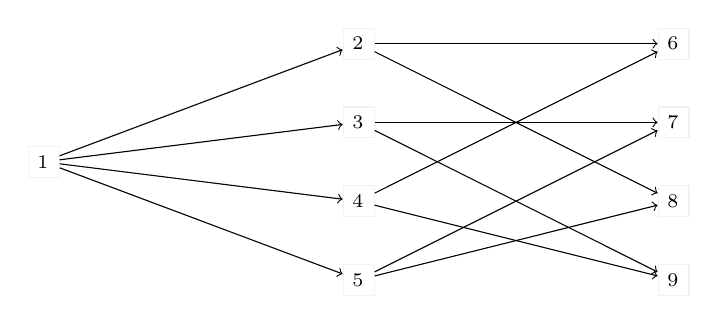
\begin{tikzpicture}
\draw (0,-3.5) node [rectangle,draw=gray!10,minimum height=0.2cm, minimum width=0.2cm, text centered] (I-1) {$\CalI_1$};

\foreach \id in {2,...,5}
	\draw (4,-\id) node  [rectangle,draw=gray!10,minimum height=0.2cm, minimum width=0.2cm, text centered] (I-\id) {$\CalI_\id$};
	
\foreach \id in {6,...,9}
	\draw (8,-\id+4) node  [rectangle,draw=gray!10,minimum height=0.2cm, minimum width=0.2cm, text centered] (I-\id) {$\CalI_\id$};
	
\foreach \id in {2,...,5} 
	\path[->] (I-1) edge (I-\id);

\path[->] (I-2) edge (I-6);
\path[->] (I-2) edge (I-8);
\path[->] (I-3) edge (I-7);
\path[->] (I-3) edge (I-9);
\path[->] (I-4) edge (I-6);
\path[->] (I-4) edge (I-9);
\path[->] (I-5) edge (I-7);
\path[->] (I-5) edge (I-8);

\end{tikzpicture}
\end{center}

Let us compute $\Phi_\CalP$ with $\CalI_1 = \langle \emptyset, \emptyset \rangle$:
\[
\begin{array}{lclcl}
\Phi_\CalP(\CalI_1) & = & \langle \{b\}, \emptyset \rangle & = & \CalI_4, \\
\Phi_\CalP(\CalI_4) & = & \langle \{a, b\}, \emptyset \rangle & = & \CalI_6, \\
\Phi_\CalP(\CalI_6) & = & \langle \{a, b\}, \emptyset \rangle & = & \CalI_6.
\end{array}
\]
The interpretation $\CalI_6$ is least fixed point of $\Phi_\CalP$, e.g. $\Lfp \Phi_\CalP = \CalI_6$, which also corresponds to the least model of $\WComp\CalP$.
\end{example}
\end{tcolorbox}
\vspace*{\fill}
\newpage

For a given set of candidate explanations $\CalC$, the set of positive candidate explanations, denoted by $\CalC^{pos}$, among the set of candidates is defined as  
\[
\begin{aligned}
\CalC^{pos} = \{\CalC_j \ | \ \CalC_j \in \CalC \mbox{ and } \CalP \cup \CalC_j \ModelsWCS \CalO\}.
\end{aligned}
\]
The set of negative candidate explanations, denoted by $\CalC^{neg}$, is given by $\CalC\setminus\CalC^{pos}$.
\end{definition}
\bigskip
\begin{prop} 
\label{prop:p0}
\normalfont
Let $\langle \CalP, \CalA_\CalP, \ModelsWCS \rangle$ be an \textit{abductive framework}, $\CalO$ an observation, and $\CalE \subseteq \CalA_\CalP$ an explanation for $\CalO$ which contains a complementary pair $c \leftarrow \top, c \leftarrow \bot$. Then, $\CalE'= \CalE \setminus \{c \leftarrow \bot\}$ is also an explanation for $\CalO$ and $\CalM_{\CalP \cup \CalE} = \CalM_{\CalP \cup \CalE'}$.
\begin{proof}
 \cite{corepaper}.
\end{proof}
\end{prop}
\bigskip
\begin{prop}
\label{prop:monotonicity}
\normalfont
Explanations are \textit{monotonic}. Let $\langle \CalP, \CalA_\CalP, \ModelsWCS \rangle$ be an abductive framework and $\CalO$ an observation. If $\CalE$ is an explanation for $\CalO$, then any set $\CalE'$ such that $\CalE \subseteq \CalE' \subseteq \CalA$ is also an explanation for $\CalO$.
\begin{proof}
\cite{holldobler2009logic}.
\end{proof}
\end{prop}

There are two possible ways of abductive reasoning: credulous and sceptical. In credulous reasoning all the consequences which follow from the program and at least one of the explanations for the observation are valid conclusions. On the other hand, in sceptical reasoning, a conclusion is only valid if it follows from the program and all the explanations for the observation. 

Let $\langle \CalP, \CalA_\CalP, \CalIC, \ModelsWCS\rangle$ be an abductive framework, $\CalO$ an observation and $\CalF$ a formula:
\begin{itemize}
\item $\CalF$ follows credulously from $\CalP$ and $\CalO$  if and only if there exists an explanation~$\CalE$ for $\CalO$ such that $\CalP \cup \CalE \ModelsWCS \CalF$.
\item $\CalF$ follows sceptically from $\CalP$ and $\CalO$ if and only if for all explanations~$\CalE$ for $\CalO$ we find $\CalP \cup \CalE \ModelsWCS \CalF$.
\end{itemize}

The set of sceptical consequences $\CalS_{\CalE}$ of a given set of explanations $\CalE$ is defined as follows
\[
\begin{array}{lcl}
\CalS_{\CalE} & = &  \underset{\CalE' \in \CalE}{\cap} \CalM_{\CalP \cup \CalE' } \\
		      & = &  \langle  \underset{\CalE' \in \CalE}{\cap} \CalM_{\CalP \cup \CalE' }^\top, \underset{\CalE' \in \CalE}{\cap} \CalM_{\CalP \cup \CalE'} ^ \bot \rangle.
\end{array}
\]

All the notions about the abductive framework, including the definition of candidate explanations and how to reason with respect to the weak completion of programs is presented in more details by Example~\ref{example:abduction} on page~\pageref{example:abduction}.

\subsection{Complexity}

\begin{prop}
\label{prop:hasexp}
\normalfont
Computing $\Lfp \Phi_\CalP$ can be done in polynomial time for acyclic logic programs $\CalP$.
\begin{proof}
See \cite{saldanha1872contextual}, Proposition 12.
\end{proof}
\end{prop}

\begin{prop}
\label{prop:hasexp}
\normalfont
Deciding whether an observation $\CalO$ has an abductive explanation based on a given program $\CalP$ and its respective set of abducibles~$\CalA_\CalP$ is NP-complete.
\begin{proof}
See \cite{saldanha1872contextual}, Proposition 13.
\end{proof}
\end{prop}

\begin{prop}
\label{prop:np}
\normalfont
Deciding whether $\CalP \cup \CalE \ModelsWCS \CalF$ does not hold for all explanations $\CalE$ given $\CalA_\CalP$ is NP-complete.
\begin{proof}
See \cite{saldanha1872contextual}, Proposition 14.
\end{proof}
\end{prop}

\begin{prop}
\label{prop:complement}
\normalfont
Let $\CalL \subseteq \sum^*$ be a language. Then $\CalL$ is NP-complete if and only if $\CalL$ is coNP-complete.
\begin{proof}
See \cite{papadimitriou2003computational}, Proposition 10.1.
\end{proof}
\end{prop}

\begin{prop}
\label{prop:hasexp}
\normalfont
Deciding whether $\CalP \cup \CalE \ModelsWCS \CalF$ holds for all explanations $\CalE$ given~$\CalA_\CalP$ is coNP-complete.
\begin{proof}
The opposite problem is shown to be NP-complete by Proposition~\ref{prop:np}. By Proposition~\ref{prop:complement}, deciding the above problem is coNP-complete.
\end{proof}
\end{prop}

\begin{definition}
\label{def:dp}
\normalfont
 A Language $\CalL$ is in the complexity class DP if and only if there are two languages $\CalL_1 \in \mbox{ NP}$ and $\CalL_2 \in \mbox{ coNP}$ such that $\CalL = \CalL_1 \cap \CalL_2$.
\end{definition}

\begin{prop}
\label{prop:hasexp}
\normalfont
The question whether $\CalF$ follows sceptically from an abductive problem is DP-complete.
\begin{proof}
See \cite{saldanha1872contextual}, Proposition 17.
\end{proof}
\end{prop}

\newpage
\vspace*{\fill}
\begin{tcolorbox}
\begin{example}
\label{example:abduction}
\normalfont
Consider program $\CalP$ consisting of the following clauses:
\[
\begin{array}{lcl}
c \leftarrow a. \\
c \leftarrow b.
\end{array}
\]
Assume that $\CalIC = \emptyset$ and that $\CalO = \{c\}$. Let us consider this observation in the abductive framework $\langle \CalP, \CalA_\CalP, \CalIC, \ModelsWCS\rangle$, where the set of abducibles $\CalA_\CalP$ consists of the following facts and assumptions:
\[
\begin{array}{ccccccc}
a &\leftarrow& \top. &\quad& a &\leftarrow& \bot.\\
b &\leftarrow& \bot. &\quad& b &\leftarrow& \bot.
\end{array}
\]
There are the following five non-complementary explanations for $\CalO$:
\[
\begin{array}{lcl}
\CalE_1 &=& \{a\leftarrow \top\}, \\
\CalE_2 &=& \{b \leftarrow \top\}, \\
\CalE_3 &=& \{a \leftarrow \top, b \leftarrow \bot\}, \\
\CalE_4 &=& \{a \leftarrow \bot, b \leftarrow \top\}, \\
\CalE_5 &=& \{a \leftarrow \top, b \leftarrow \top\}.
\end{array}
\]
The only minimal explanations for $\CalO$ are $\CalE_1$ and $\CalE_2$. As $a$ and $b$ does not follow from all the explanations, it does not follow sceptically, but only credulous, from $\CalP$ and $\CalO$. \\
\newline
The set of candidate explanations $\CalC$ for $\CalP$ and $\CalO$ is the power set of $\CalA_\CalP$. The set of non-complementary candidate explanations $\CalC_{\CalA_\CalP}^{nc}$ consists of the following nine candidates:
\[
\begin{array}{lcl}
\CalC_1 = \emptyset, &\quad\quad& \\
\CalC_2 = \{a \leftarrow \top\}, &\quad\quad& \CalC_2 = \{a \leftarrow \bot\}, \\
\CalC_4 = \{b \leftarrow \top\}, &\quad\quad& \CalC_5 = \{b \leftarrow \bot\}, \\
\CalC_6 = \{a \leftarrow \top, b \leftarrow \top\}, &\quad\quad& \CalC_7 = \{a \leftarrow \top, b \leftarrow \bot\}, \\
\CalC_8 = \{a \leftarrow \bot, b \leftarrow \top\}, &\quad\quad&\CalC_9 = \{a \leftarrow \bot, b \leftarrow \bot\}. \\
\end{array}
\]
The set of minimal candidate explanations for $\CalA_\CalP$ and $\CalO$, $\CalC_{\CalA_\CalP,\CalO}^{min}$, consists of the candidates $\CalC_1$, $\CalC_2$, $\CalC_3$, $\CalC_4$, $\CalC_5$ and $\CalC_9$. The set of positive candidate explanations $\CalC_{\CalA_\CalP,\CalO}^{min, pos}$ consists only of $\CalC_2$ and $\CalC_4$. Finally, the sceptical consequences of $\CalC_{\CalA_\CalP,\CalO}^{min, pos}$ is given by
\[
\CalS_{\CalC_{\CalA_\CalP,\CalO}^{min, pos}} = \langle \{a, c\} \cap \{b, c\}, \emptyset \cap \emptyset \rangle = \langle \{c\}, \emptyset \rangle
\]
\end{example}
\end{tcolorbox}
\vspace*{\fill}
\newpage

% -------------------------------------------------------------------------------------------------------------------------------------------------------------------------------------------------------------------------------------------------------------------------------------------- %
\section{Connectionist Networks}
\label{sec:preliminaries:cn}

A connectionist network consists of interconnected processing units. The general model of a processing unit consists of a summing part followed by an output part. The summing part receives N input values, weights each value, and computes a weighted sum. The weighted sum is called the \textit{activation value}. The sign of the weight for each input determines whether the input is \textit{excitatory} (positive weight) or \textit{inhibitory} (negative weight). The output part produces a signal from the activation value. 

We can divide these connectionist networks into two large classes. One class consists of the feed-forward networks and the other class consists of the recurrent networks. In general, whether a network belongs to one class or another can be decided based on its overall connectivity. If the network has one or more cycles, i.e., it is possible to follow a path from a unit to itself, then the network is referred to as recurrent. Feed-Forward networks have no cycles. 

We assume the reader to be familiar with connectionist networks as, for example, it is defined in \cite{feldman1982connectionist}. In particular, we will use McCulloch-Pitts networks of threshold units as defined in \cite{mcculloch1943logical} and multi-layer feed-forward networks as defined in \cite{rumelhart1986general}. We use modified connections of the following form:

\begin{itemize}

\item In case of a \textit{positively modified connection}, the input $i = wv$ of a unit is only received if the modifier $m$ is $1$, where $v$ is the output of the sending unit and $w$ is the weight of the connection:
\[
i = \left\{ 
\begin{array}{ll}
wv & \mbox{if } m=1, \\
0   & \mbox{if } m=0.
\end{array}
\right .
\]

\item In case of a \textit{negatively modified connection}, the input $i = wv$  is only received if the modifier $m$ is $0$:
\[
i = \left\{
\begin{array}{ll}
0 & \mbox{if } m=1, \\
wv & \mbox{if } m=0.
\end{array}
\right .
\]
\end{itemize}

The modifier $m$ is the output of another unit. Figure~\ref{fig:modifier} shows the graphical representations of a positively and a negatively modified connection. 

\begin{figure}
	\centering
	\begin{subfigure}{0.45\textwidth}
		\scalebox{.8}{\modifiedconnectionspassive}
  		 \caption{Negative modification.}
	\end{subfigure}
	\hspace{1cm}
	\begin{subfigure}{0.45\textwidth}
		\scalebox{.8}{\modifiedconnectionsactive}
   		\caption{Positive modification.}
	\end{subfigure}
	\caption{The output $v$ of unit $u_1$ is received by the input $i$ of unit $u_2$ only if the modifier $m$ of unit $u_3$ is 0 (a) or 1 (b), respectively.}
	\label{fig:modifier}
\end{figure}

\subsection{Recurrent Networks}
\label{sec:preliminaries:rcn}

The following notions introduced here are based on \cite{hertz1991introduction, medsker1999recurrent}. If the input in a feed-forward network is held constant, the trajectory of the network in state space will remain at a single point. Clearly, in order to archive interesting sequential behaviour in the presence of a constant input, there must be recurrent connections in the network. Therefore, because our main goal is to generate a sequence of candidate explanations for the abductive framework which characterises a sequential behaviour, we will focus on recurrent networks.

Recurrent networks were created in the 1980's and have been an important focus of research and development during the 1990's. They are designed to learn sequential or time-varying patterns, because each unit can use its internal memory to maintain information about the previous input. In cases of language, for example, if we would like to predict the next word in a sentence it is very important to know which words came before it. Thus, allowing the network to gain a deeper understanding of the statement is a great property when it comes to problems like this one. Language modelling is only one of the many applications for these recurrent networks. They have also been applied to image processing, pattern recognition, classification, clustering, data mining and so on.

The topology of a recurrent network can be very general, since they allow feedback connections. This means that every unit can be connected to every unit, including to itself. Allowing the presence of feedback connections among units brings an important characteristic to this networks, a time-dependent behaviour. Because of this, they can also be classified as dynamic networks. The state of a network, at one moment in time, also depends on the state at a previous moment in time. The dynamics of a recurrent neural network can be continuous or discrete in time. When a continuous time system is simulated, it is usually converted into a set of simple first order difference equations, which is formally identical to a discrete system. Therefore, we will concentrate on discrete time networks.

The dynamics of a recurrent network can be described, for instance, by a discrete time system 
\[
x(k + 1) = f(x(k)), \quad k \geq 1, 2,...,
\]
where $x$ denotes the state of the corresponding network and $f$ is some suitable mapping. 

The architecture of the recurrent network can vary from fully interconnected (Figure~\ref{fig:fullyconnected}) to partially connected (Figure~\ref{fig:partiallyconnected}). Fully connected networks do not have distinct input layers of nodes, and each unit has a weighted connection to every other unit in the architecture as well as a single feed-back connection to itself.

Simple partially recurrent networks (Figure~\ref{fig:partiallyconnected}) have distinct input layer of nodes and not every unit must be connected to every other unit. However, although some nodes are part of a feed-forward structure, other units provide the sequential context and receive feed-back connections from other units. These units are denoted the context units and composed what we will later refer to as the context layer. Weights from the context units (e.g., C1 and C2 in out example) are processed like those for the input units, for example, using back propagation. The context units receive time-delayed feedback from, in the case of Figure~\ref{fig:partiallyconnected}, the second layer units. Training data consists of inputs and their desired successor outputs. These type of networks can be trained, for example, to predict the next letter in a string of characters or to validate a string of characters.

\begin{figure}
	\centering
	\begin{subfigure}[b]{0.7\textwidth}
		\centering
		\scalebox{1.0}{\fullyconnected} 
		\bigskip
		\caption{\label{fig:fullyconnected} Fully connected.}
	\end{subfigure}
	\par\bigskip\par\bigskip\par\bigskip
	\begin{subfigure}[b]{0.7\textwidth}
		\centering
		\scalebox{1.0}{\partiallyconnected} 
		\bigskip
		\caption{\label{fig:partiallyconnected} Partially connected.}
	\end{subfigure}
	\par\bigskip
	\caption{Examples of a fully connected (a) and a partially connected (b) recurrent network. Solid lines represent trainable connections.}
\end{figure}

Back-propagation in feed-forward networks moves backward from the final error through the outputs, weights and inputs of each hidden layer, assigning those weights responsibility for a portion of the error by calculating their partial derivatives. These derivatives are then used by the learning rule, e.g. gradient descent, to adjust the weights up or down, depending on which direction decreases error.

Recurrent networks rely on an extension of back-propagation called back-propagation through time. Time, in this case, is simply expressed by a well-defined, ordered series of calculations linking one time step to the next, which is all back-propagation needs to work. Note that, Neural Networks, recurrent or not, are simply nested composite functions like $f(g(h(x)))$. Adding a time element only extends the series of functions for which we calculate derivatives with the chain rule.

In the sequel, the algorithm used will be the one developed in \cite{rumelhart1986leanrning}. The algorithm is a gradient search in weight space for a set of weights which implements the desired function. In \cite{rumelhart1986leanrning} the algorithm is demonstrated for nonrecurrent networks, but it can also be applied to recurrent networks.

To illustrate some of the ideas introduced here, a simple partially connected Recurrent Network consisting of two units is shown in Example~\ref{example:simplern} on page~\pageref{example:simplern}. Now we will now introduce two fundamental ways which can be used to add feed-back into feed-forward multi-layer networks, i.e. Jordan Networks and Elman networks. 

\subsection{Jordan Networks}
\label{sec:preliminaries:nn:jordan}

A theory of serial order which describes how sequences of actions might be learned and performed is presented in \cite{jordan1997serial}. The theory is embodied in the form of a parallel distributed processing \cite{rumelhart1986parallel} or connectionist network \cite{feldman1982connectionist}. Such networks are composed of many simple processing units that are connected though weighted links. The structure of the network consists of plan units, state units, hidden units and output units. The plan units and the state units together serve as the input units for a network which implements the output function $f$ through weighted connections from the plan and state units to the output units. The next-state function is implemented with recurrent connections from the output units to the state units. This allows the current state to depend on the previous state and on the previous output (which is itself a function of the previous state and the plan). The full overall structure of the network is shown in Figure~\ref{fig:jordan}.

In the proposed network, there is no explicit representation of temporal order and no explicit representation of action sequences. This is due to the fact that there is only one set of output units for the network, so that at any point in time, only one output vector is present. The network proposed by Jordan essentially implements the output function which relates patterns as a network associative memory in which many associations are stored in the same set of weights. The learning and generalisation of abilities demonstrated for such networks \cite{rumelhart1986parallel, rumelhart1981parallel} are just those that are needed for the output function.

Although it is possible that the next-state function is learned, this is not necessary for the system as a whole to be able to learn to produce sequences. Therefore, the recurrent connections have a fixed weight of 1.0 and all the other connections are trained. Learning is realised as an error-correcting process in which parameters of the network are incrementally adjusted based on the difference between the actual output of the network and the desired output. Essentially, the next-state function provides a time-varying state vector, and associations are learned from this state vector and plan vector to desired output vectors. 

The form that desired output vectors are assumed to take is a generalisation of the approach used in traditional error-correlation schemes. Instead of assuming that a value is specified for each output unit, it is assumed that there are constraints specified on the values of the output units. Constraints may specify a range of values that an output unit may have, a particular value, or no value at all. It is also possible to consider constraints that are defined among output units. For example, the sum of the activations of a set of units might be required to take on a particular value. More details on how these constraints enter into the learning process is given in \cite{jordan1997serial}.

\begin{figure}
\centering
\scalebox{1.0}{\jordangeneral}
\caption{\label{fig:jordan}A simple recurrent network in which activations are copied from the output layer to the context layer on a one-for-one basis, with fixed weight of 1.0. Solid lines represent trainable connections.}
\end{figure}

\subsection{Elman Networks}
\label{sec:preliminaries:nn:elman}

As introduced in \cite{elman1989representation} and \cite{elman1990finding}, an Elman Network is a three-layered recurrent network, with an additional set of units called the context layer. Both the input units and the context units activate the hidden units. The hidden units then feed forward to activate the output units and also feed back to activate the context units. This constitutes the forward activation. The output is then compared with the expected output for the given input and back propagation is used to adjust connection strengths incrementally. Recurrent connections are fixed at 1.0 and are not subject to adjustments.  The full overall structure of the network is shown in Figure~\ref{fig:elman}.

As one may notice, this approach is an variation of the Jordan Networks introduced in the previous Section. The only difference between them is on the source of the recurrent connections, which is the output layer and the hidden layer for Jordan and Elman networks, respectively. This is also the main characteristic of the Elman networks, which is an internal representation of time.

\newpage
\vspace*{\fill}
\begin{tcolorbox}
\begin{example}
\label{example:simplern}
\normalfont
An example of a simple partially connected recurrent network consisting of two units is shown below. 
\begin{center}
\scalebox{1.0}{\simplernn}
\end{center}
The recurrent connection of the output unit back to itself means that the output of the network depends not only on the input, but also on the state of the network at the previous time step.
\bigskip

For example, letting $\mu$ be the value of the recurrent weight, and assuming for simplicity that the units are linear ,i.e., the function is the identity function, the activation of the output unit at time t is given by
\[
x_2(t) = \mu x_2(t-1) + w_{21}x_1(t)
\]
where $x_1(t)$ is assumed to be constant over time. \\
\end{example}
\end{tcolorbox}
\vspace*{\fill}
\newpage

In feed-forward networks employing hidden units and a learning algorithm, the hidden units develop internal representations for the input patterns that recode those patterns in a way which enables the network to produce the correct output for a given input. In the architecture presented in \cite{elman1989representation}, the context units remember the previous internal state. Therefore, the hidden units have the task of mapping both an external input and the previous internal state to the desired output. Because the patterns on the hidden units are saved as context, the hidden units must accomplish this mapping and at the same time develop representations which are useful encodings of the temporal properties of the sequential input. Thus, the internal representations are now sensitive to temporal context.

\begin{figure}
\centering
\scalebox{1.0}{\elmangeneral}
\caption{\label{fig:elman}A simple recurrent network in which activations are copied from the hidden layer to the context layer on a one-for-one basis, with fixed weight of 1.0. Solid lines represent trainable connections.}
\end{figure}